\chapter{Implementation}\label{ch:impl}

The system is implemented in Python (protocol, simulation glue, detection and evaluation), Go
(chaincode) and JavaScript (ledger gateway and live map). Everything is in one repository and runs
from a Makefile. This chapter describes the parts and how they connect.

\section{Overview}

\begin{figure}[htbp]\centering
\begin{tikzpicture}[
  box/.style={draw, rounded corners, align=center, minimum height=1.05cm, text width=3.0cm, font=\small},
  arr/.style={-{Latex[length=2mm]}, thick}]
  \node[box, fill=gray!10] (sumo) at (0,0) {SUMO\\\scriptsize grid or LuST traffic};
  \node[box, fill=blue!8] (ns3) at (4.5,0) {ns-3 802.11p\\\scriptsize who hears what, when};
  \node[box, fill=orange!10] (proto) at (9,0) {Protocol\\\scriptsize vehicle and RSU apps};
  \node[box, fill=green!8] (ledger) at (9,-2.3) {Ledger\\\scriptsize mock or Fabric gateway};
  \node[box, fill=red!8] (det) at (4.5,-2.3) {Detector\\\scriptsize rules / learned};
  \node[box, fill=gray!10] (metrics) at (0,-2.3) {metrics.csv,\\\scriptsize protocol\_stats.json};
  \node[box, fill=yellow!15] (eval) at (0,-4.6) {collect, report,\\\scriptsize plots, results page};
  \node[box, fill=yellow!15] (viz) at (4.5,-4.6) {live narration\\\scriptsize and browser map};
  \draw[arr] (sumo) -- node[above, font=\scriptsize]{ns-2 trace} (ns3);
  \draw[arr, <->] (ns3) -- node[above, font=\scriptsize]{packets} (proto);
  \draw[arr, <->] (proto) -- (ledger);
  \draw[arr, <->] (proto) -- (det);
  \draw[arr] (proto.south west) -- (metrics.north east);
  \draw[arr] (metrics) -- (eval);
  \draw[arr] (metrics) -- (viz);
\end{tikzpicture}
\caption{Simulation and evaluation pipeline}\label{fig:pipeline}
\end{figure}

Figure~\ref{fig:pipeline} shows the pipeline. SUMO~\cite{lopez2018sumo} decides where every vehicle drives. ns-3 models
the radio: transmission, propagation, collisions and the MAC. The protocol code runs inside every
vehicle and RSU node and talks to the ledger and the detector. Every event is logged to
\texttt{metrics.csv}, from which the evaluation computes all results. Table~\ref{tab:code} lists
the main parts of the code.

\begin{table}[htbp]\centering\small
\caption{Code organisation}\label{tab:code}
\begin{tabular}{@{}lp{10.5cm}@{}}
\toprule
Folder & Contents \\
\midrule
\texttt{mobility/} & grid and LuST scenario builders, SUMO-to-ns-2 trace conversion, RSU placement \\
\texttt{network/} & scenario runner, ns-3 radio backend, node hooks, metrics, ledger bridge, live map \\
\texttt{protocol/} & vehicle and RSU logic, cryptography, message encoding, registration, escrow, TESLA, ECQV, Bloom filter, batch verification, V2V verifier, simulator glue \\
\texttt{ledger/} & Fabric network scripts, Go chaincode, Node.js REST gateway, mock ledger, conformance tests, load benchmark \\
\texttt{detection/} & detector (rules, features, learned models), VeReMi loaders, benchmark and training \\
\texttt{experiments/} & sweep configurations, runner, collection, reports, plots, results page, tracker attack \\
\bottomrule
\end{tabular}
\end{table}

\section{Mobility}

\textbf{Grid.} A $5\times5$ junction grid with 250\,m blocks (1\,km$^2$) and two lanes per
direction. Random trips start during the first half of the run, so vehicles enter one after another.
Nine RSUs stand 450\,m apart, each with a nominal range of 300\,m, so ranges overlap.

\textbf{LuST.} The Luxembourg SUMO Traffic scenario~\cite{codeca2015lust} models a full day of the
city's traffic. The evaluation simulates the whole city and cuts a 1.35\,km\,$\times$\,1.35\,km box
in the centre at three times of day: 06:00 (about 150 vehicles in the box), 14:00 (about 260) and the
08:00 peak (about 525). A 900\,s warm-up fills the roads before the measured window. Vehicles that
leave the box are parked outside radio range until they come back.

\textbf{Mobility step and lane changes.} SUMO runs at 0.1\,s steps. Its default instant lane change
is a 3.2\,m sideways jump in one step, which the trace turned into a false 32\,m/s velocity that the
detector rightly flagged. The evaluation therefore uses a 2\,s lane-change duration, as real drivers
do, which removed all such spikes on the grid and all but two of 385 on LuST.

\section{Radio Network}

\begin{table}[htbp]\centering\small
\caption{IEEE 802.11p parameters in ns-3}\label{tab:radio}
\resizebox{\textwidth}{!}{%
\begin{tabular}{@{}lp{9cm}@{}}
\toprule
Parameter & Value \\
\midrule
Standard, band & IEEE 802.11p (WAVE), 5.9\,GHz, 10\,MHz channel \\
Data rate & 6\,Mb/s \\
Transmit power, receiver sensitivity & 20\,dBm, $-85$\,dBm \\
Propagation & log-distance, exponent 2.196, 47.86\,dB at 1\,m \\
Nominal range & 400\,m \\
Access categories & BSMs, beacons and TESLA keys on AC\_VO; the rest on AC\_BE \\
Wired RSU backbone & 2\,ms latency \\
\bottomrule
\end{tabular}}
\end{table}

ns-3 (version 3.44~\cite{riley2010ns3}) is driven from Python through its cppyy bindings.
Table~\ref{tab:radio} lists the radio configuration. A lighter pure-Python backend with the same
parameters exists for development and unit tests; every reported result comes from ns-3. ns-3's
FlowMonitor and the PHY's busy time give the delivery ratio and the channel busy ratio, sampled every
second at each RSU.

\section{Protocol}

The protocol package implements Chapter~\ref{ch:design}. Schnorr signatures and
proofs use \texttt{coincurve} (libsecp256k1), and the escrow uses AES-GCM~\cite{nist80038d} from
\texttt{cryptography}. Messages use a compact binary encoding: one byte per field
name from an append-only table, binary hex strings, and 16-byte packed kinematics. Vehicles and RSUs
are applications attached to ns-3 nodes through a small set of hooks: send, schedule, position, log
and the local ledger copy.

\textbf{Processing time.} Simulated time does not advance while Python computes. Instead, the cost of
every cryptographic operation was measured on the real implementations
(Table~\ref{tab:compute}) and is charged as processing delay. With \emph{per-node processor} modelling, each
RSU and vehicle has one processor that executes this work in arrival order. Latency therefore
includes queueing, and a BSM that would wait more than 100\,ms is dropped as too old to be useful.
Vehicle processors are assumed five times slower than the development PC, an AMD Ryzen~7 4800H. A
sensitivity sweep varies this factor (Section~\ref{sec:res-sens}).

\gentab{tab_compute}

\textbf{Vehicle-side verification.} Each vehicle verifies the BSMs of senders within 100\,m on its
own processor, as a receiver that acts on them would. It caches tickets learned from full-ticket BSMs
of farther senders.

\section{Ledger}

The chaincode is written in Go for Hyperledger Fabric~3.1.5 and deployed on a Fabric network with two
peer organizations and an ordering service of one Raft orderer or four SmartBFT orderers. A Node.js
gateway exposes it as a REST interface. It maps an \texttt{X-Identity} header to the caller's Fabric
certificate, signs transactions, reports endorsement and commit times, and keeps an activity log. An
HTTP conformance suite runs unchanged against the real gateway and against a mock with the same
rules. For long parameter sweeps, the simulator uses an in-process ledger with the same functions
and a 500\,ms commit delay, which is the Raft commit time measured with the default batch timeout
(Section~\ref{sec:res-ledger}). RSUs read from a local copy that is updated every second, or at the
mock's commit time.

\section{Detection}

The detector computes per-message plausibility features against the pseudonym's history: implied
speed, speed and position consistency over 0.8--3\,s baselines, acceleration, heading change,
message rate, distance from the RSU, the signal-strength distance and sequence numbers. It applies the
rules of Section~\ref{sec:detect}. For comparison, learned models over the same features (a random
forest and gradient-boosted trees~\cite{friedman2001gbm} with a history window, built with
scikit-learn~\cite{pedregosa2011sklearn}) are trained and tested on VeReMi
Extension~\cite{kamel2020veremiext}, on five vehicle-disjoint splits so that no vehicle's messages
appear in both training and test data. The scheme itself uses the rules and the signal-strength
check, which do not depend on the road network.

\section{Evaluation Framework}\label{sec:eval-framework}

A sweep is a JSON configuration: fixed options, a grid of parameters (for example 50, 100 and 150
vehicles), the variants to compare and the seeds. The runner executes every combination in parallel
and skips finished runs. A collection step turns each run's event log into about 100 metrics. The
report step computes means with 95\,\% confidence intervals over the seeds and Welch's
t-test~\cite{welch1947} against each baseline, and writes Markdown and LaTeX tables, PNG, PDF and SVG
figures, and an interactive results page. The tables and numbers in this report are generated from
the same outputs (Appendix~\ref{app:repro}).

\textbf{Baselines.} Two baselines run on the same simulator. \emph{ECDSA-PKI} represents IEEE
1609.2-style pseudonym certificates: the vehicle presents a CA-signed certificate and signs with
ECDSA~\cite{johnson2001ecdsa} P-256, using the measured ECDSA costs. \emph{Central-TA} sends every login over the backbone
to one central authority that decides and answers.

\textbf{Tracker.} For privacy, a global eavesdropper records every BSM. A tracker then tries to link
each new pseudonym to a disappearing one by predicting positions from the last speed and heading. The
metrics are the share of pseudonym changes linked correctly and the share of a trip that can be
followed from start to end.

\section{Live Demonstration Tools}

Two tools show a run as it happens. A terminal narration prints each important event in plain
language, with a one-line explanation the first time each kind appears, and a status line every five
simulated seconds. A live map in the browser (Figure~\ref{fig:livemap}) draws the SUMO road network,
the RSUs with their coverage and every vehicle, coloured by its state. Clicking a vehicle shows its
pseudonym, class, ticket, revocation state and recent events. Clicking an RSU shows its load, the
vehicles in range, its counters and its recent checks. The page can pause the simulation and change
its speed.

\begin{figure}[htbp]\centering
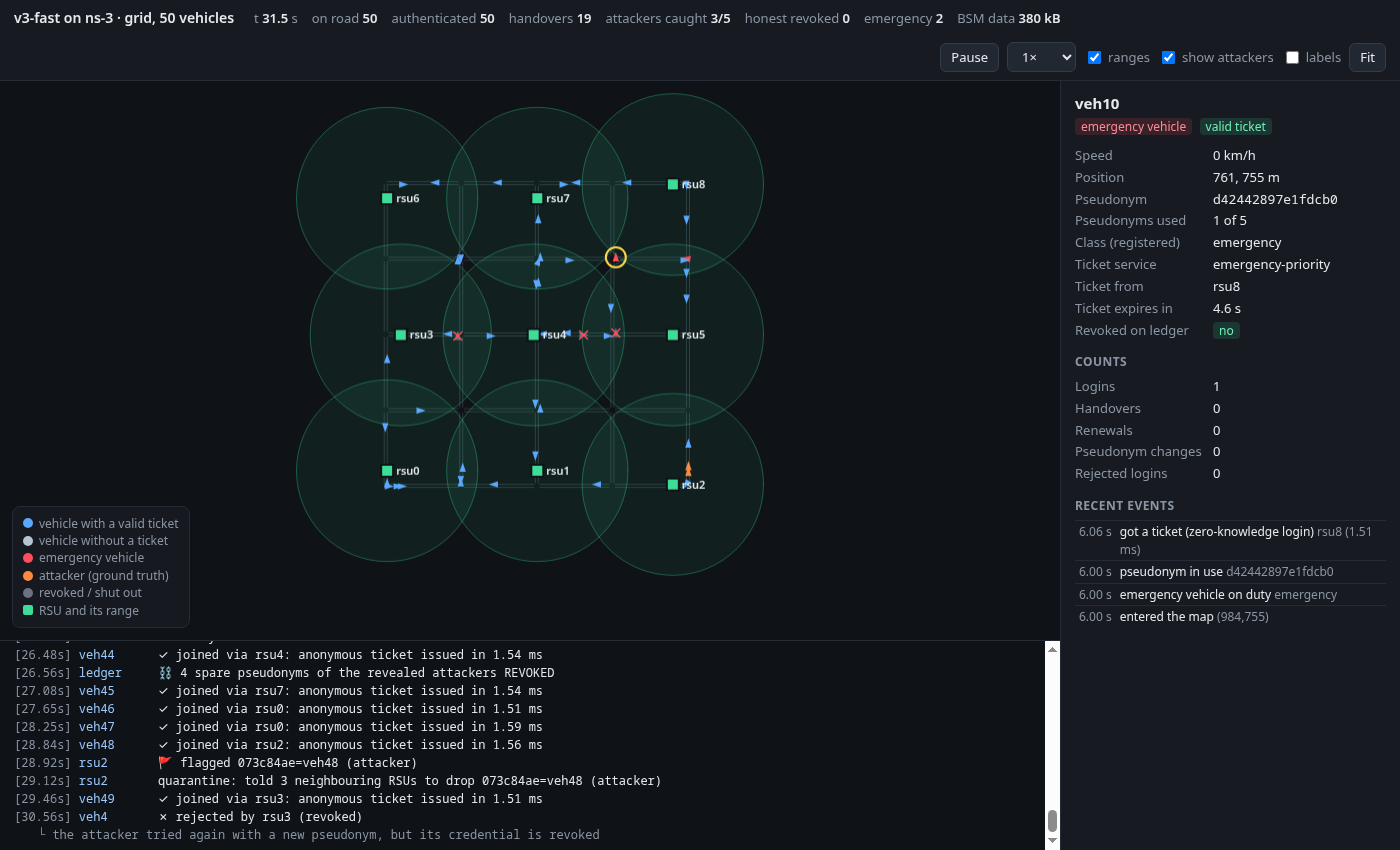
\includegraphics[width=0.85\textwidth]{figures/live_map_vehicle.png}
\caption{Live map of a running ns-3 simulation (grid, 50 vehicles, with emergency vehicles).
The selected emergency vehicle shows its registered class and its \texttt{emergency-priority}
ticket; revoked attackers are marked with a cross; the feed narrates detection and revocation.}
\label{fig:livemap}
\end{figure}

\section{Testing}

178 automated tests cover the cryptographic primitives, message encoding, the protocol flows
(including replay, forged tickets, swapped certificate requests, class escalation and fake emergency
alerts), the detector, the ledger rules and the processor model. The chaincode has its own Go unit
tests, and the gateway passes the HTTP conformance suite.
